%!TEX root = ../fbi.tex

\section{Entanglement spectrum}
\label{sec:ES}

The quasi-1D cylinder geometry is also convenient for calculating the 
entanglement spectrum for entanglement cuts transverse to the 
cylinder. With each cylinder slice blocked together and considered as an MPS, the procedure for computing the entanglement spectrum is identical to those used for MPS. The process also results in a change of basis on the virtual legs that allows one to change the tensor network in Figure \ref{fig:FBI_PEPS} into a canonical form MPS,

$$
\ket{\psi} = \sum\limits_{\{p_i\}} \ldots \Lambda \Gamma_{p_0} \Lambda \Gamma_{p_1} \Lambda \Gamma_{p_2} \Lambda \ldots \ket{... p_0 p_1 p_2 ...}.
$$

Each physical leg represents all $2L$ physical indices of a cylinder slice, 
and each virtual leg represents all $L$ virtual indices that connect cylinder 
slices. The change of basis generally mixes the Hilbert spaces from these 
virtual legs, so the resulting basis won't be local around the circumference 
of the cylinder.
For many of the calculations that follow, we'll use this 1D form, and the 
methods will be entirely MPS methods. 

As is well known, the key property of the canonical form is that it provides a Schmidt decomposition $\ket{\psi} = \sum\limits_i \ket{\psi_L^i} \lambda_i \ket{\psi_R^i}$, as shown in Figure \ref{fig:mps_canonical}. The Schmidt vectors $\ket{\psi_{L/R}^i}$ make an orthonormal set of eigenvectors for the reduced density matrices $\rho_{L/R}$ of the left/right half of the system. 

\begin{figure}[htbc]
	\centering
		\includegraphics[width=0.8\columnwidth]{{mps_canonical.pdf}}
		\caption{}
		\label{fig:mps_canonical}
\end{figure}

This Schmidt decomposition only has a finite number $\chi$ of contributing 
terms - one for each non-zero eigenvalue $\rho_i = \lambda_i^2$ of the reduced 
density matrices on either side of the cut -
which is bounded by the total bond dimension crossed by the 
entanglement cut.  For the HFBI and the cut shown in Figure 
\ref{fig:FBI_PEPS}, the number of terms is $2^L$. 

The entanglement Hamiltonian $H_e$ is defined via  $e^{-H_e} = \rho$,
where $\rho$ is the reduced density matrix for the half-infinite cylinder
on one side of the entanglement cut. Its eigenvectors are thus also the Schmidt
states, and its eigenvalues are $\epsilon_i =-\log \rho_i$. 
Due to the finite correlation length of the state, the
differences between the Schmidt states are exponentially localized to the 
boundary. For this reason, we refer to these states as the `entanglement 
edge'. 
 
As shown in \cite{perezgarcia2008}, a translationally invariant MPS can be
assigned a projective representation of the on-site symmetry group, acting on 
the virtual legs, that maps Schmidt states to degenerate Schmidt states. 
For the MPS formed by the HFBI, we find that the U(1) boson number symmetry 
and the$\mathbb{Z}_L$ translational symmetry around the cylinder circumference 
are represented linearly. Each Schmidt state can thus be assigned a 
well-defined quantum number of charge and transverse momentum. We'll discuss 
this assignment of charge further in \ref{sec:symmetry}.
 
The entanglement spectra for the HFBI on cylinders with even and odd width 
circumferences are shown in \ref{fig:ESL10} and \ref{fig:ESL9}, plotted 
against the transverse momentum eigenvalue and colored by the U(1) charge 
eigenvalue of the corresponding Schmidt states. 
We find that the entanglement spectrum looks like it has a gapless
edge mode with linear dispersion near momentum zero.

\begin{figure}[htbc]
	\centering
	\includegraphics[width=\columnwidth]{{EntanglementSpectrum_L10.pdf}}
	\caption{Entanglement spectrum on a zig-zag edge L=10 cylinder}
	\label{fig:ESL10}
\end{figure}


\begin{figure}[htbc]
	\centering
	\includegraphics[width=\columnwidth]{{EntanglementSpectrum_L9.pdf}}
	\caption{Entanglement spectrum on a zig-zag edge L=9 cylinder}
	\label{fig:ESL9}
\end{figure}

In figure \ref{fig:EEScaling}, we compare the lowest points in 
the spectra for several cylinder widths. The finite size scaling confirms that 
the entanglement gap closes as $1/L$, as you would expect for a gapless mode 
with linear dispersion.

\brayden{Something about history of 2d SPTs having gapless 
entanglement edges. Possibly see brayden's advancement talk.}

Gapless entanglement spectra have been shown to be robust features of 
two-dimensional topological and symmetry protected topological (SPT) phases.

\begin{figure}[htbc]
	\centering
	\includegraphics[width=\columnwidth]{{EntanglementEnergyScaling.pdf}}
  \caption{Power law fits for the lowest five states above the ground state in Figure \ref{fig:ESL10}. The 
  $1/L$ scaling is a signature of a gapless (entanglement) Hamiltonian. Due to the small system size, 
  points at non-zero momentum still deviate significantly from $1/L$ scaling.}
  \label{fig:EEScaling}
\end{figure}

\begin{figure}[htbc]
	\centering
  \includegraphics[width=\columnwidth]{{TopologicalEntanglementEntropy.pdf}}
	\caption{The topological entanglement entropy $\gamma$ is consistent 
	with 0.}
	\label{fig:TopologicalEE}
\end{figure}

The most likely explanation for this gapless edge mode is that the state has 
topological or SPT order. By computing the topological entanglement entropy, 
as shown in \ref{fig:TopologicalEE}, we can rule out 
topological order for this state. Combined with the vanishing of topological 
entanglement entropy, these spectra suggest that the 
HFBI state are in a featureless SPT phase. 


However, the entanglement spectrum of this one wavefunction is not enough to 
determine the SPT nature of the phase. First, it isn't clear what group or 
groups of symmetries can be used to protect the gapless edge. It could be that 
the entire symmetry group - $U(1)$ boson number conservation, \brayden{time 
reversal symmetry?}, as well as the entire rotational and translational group 
of the lattice - must be preserved to protect the edge. Or, as we will argue 
is the case, a much smaller subgroup could be used to protect the edge. This 
leads to a wider class of perturbations that leave the edge intact - and since 
we will argue that translation is not needed for protection, the gapless edge 
will additonally be robust to some types of weak disorder and can be seen in 
small systems with symmetry preserving boundary conditions. Second, the 
entanglement spectrum alone fails to distinguish between other SPT phases with 
the same protecting group - for that, we need a topological invariant. Third, 
we would like to confirm the SPT nature of the phase by perturbing a parent 
Hamiltonian with terms that break various combinations of symmetries and 
seeing if they destroy the gapless edge.

%To determine the protecting group, we can proceed in 
%two ways: we could perturb a parent Hamiltonian with terms that break various 
%combinations of symmetries and see which perturbations destroy the gapless 
%edge, or we can look for a topological invariant by analyzing the action of 
%the symmetry of the entanglement edge. We will take up the later question 
%first, then return to the prospect of perturbing a parent Hamiltonian in 
%Section \ref{sec:perturbations}.

Notice that many points in the spectrum are doubly degenerate - those that are 
assigned a non-zero $U(1)$ charge - and on odd circumference cylinders, the 
entire entanglement spectrum is doubly degenerate, a property shared with 1D SPTs. This suggests that the the HFBI state as a 1D state with any  
fixed odd cylinder circumference $L$ is a 1D SPT. We will discuss in
Section \ref{sec:symmetry} how to explain the degeneracies in these spectra 
using the action of the symmetry on the edge, and how to prove that the odd 
circumference cylinder states are indeed 1D SPTs while the even circumference 
cylinder states are not. This will shed light on what the appropriate symmetry 
group to use.

Given that only odd circumference cylinders are SPTs, one might wonder whether 
odd and even $L$ cylinders approach two differt phases in the thermodynamic 
limit. In Section \ref{sec:CFT}, we will provide evidence against that 
possibility, by showing that in both cases, the low-energy, linear dispersing 
part of the entanglement spectra can be described by the same conformal field 
theory. Thus, in the thermodynamic limit, the two edge spectra approach the 
same set of points.
	
\subsection{Symmetry action on the edge}
\label{sec:symmetry}

When we treat the HFBI wavefunction on a 
cylinder of a fixed circumference $L$ as a matrix product state, we can use 
MPS methods to determine the action of an on-site symmetry on 
the virtual legs of this MPS. This is done using the MPS canonical form, as 
originally detailed in \cite{perezgarcia2008}. This will allow us to determine 
the boson charge and transverse momentum associated with each Schmidt state, 
used in the spectra plots Figures \ref{fig:ESL10} and \ref{fig:ESL9}.

This symmetry action is determined on the Schmidt basis, but we can also 
change back to the basis determined by the virtual legs of the PEPS in Figure 
\ref{fig:FBI_PEPS_2}, i.e. a basis that is local around the circumference of 
the cylinder. We'll use this basis to describe the edge action of the on-site 
symmetries of the MPS: U(1) charge, translation, and reflection $I_y$. 

Each on-site symmetry of the wavefunction $U_g = \otimes_i u^i_g$, with $U_g 
\ket{\psi} = e^{i \Theta_g} \ket{\psi}$ is assigned an operator $V_g$ that 
acts on the virtual leg of the MPS, that satisfies the equation
\begin{center}
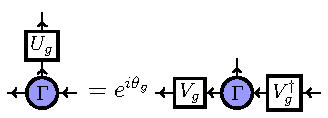
\includegraphics[width=0.6\columnwidth]{group_sym.pdf}
\end{center}

For an MPS with a nondegenerate largest 
transfer matrix eigenvalue, this equation is guaranteed have a unique solution 
for $V_g$, and the operators $V_g$ are guaranteed to commute with the diagonal 
matrix $\Lambda$. However, these operators are not guaranteed to form a linear 
representation of the group of on-site symmetries, but in general could make 
up a projective representation, satisfying 
$$V_g V_h = e^{i \omega(g, h)} V_{gh}.$$



%By combining $N$ such blocks together and connecting them with periodic 
%boundary conditions, we recover the fact that 
%$U_g \ket{\psi} = e^{i \Theta_g} \ket{\psi}$,
%with $\Theta_g = N \theta_g$, since all of the $V_g$ and $V_g^{\dagger}$s 
%cancel pairwise.
%$\theta_g$ measures the charge per unit cell
    

%In general, the $V_g$ do not have to form a linear representation of the 
%group, but could instead be a projective representation. This can be explained 
%in the MPS language as follows: if instead the blocks are connected together 
%with different boundary conditions, as in Figure \ref{fig:mps_boundary}, we 
%discover that $U_g$ transforms $\ket{\psi}$ to a similar state with 
%transformed boundary conditions, $B \rightarrow V_g^{\dagger} B V_g$. This 
%action on $B$, one can show, is a group representation.

%For open ends - if $B$ factors into left and right parts, $B = 
%\vket{b}\vbra{b}$ - the action of the symmetry on the boundary can also be 
%factored, $\vket{b} \rightarrow V_g \vket{b}$. This action does not have to be 
%a group representation, but can fail up phases $V_g V_h = e^{i \omega(g, h)} 
%V_{gh}$.  

%\begin{figure}[htbc]
%    \centering
%    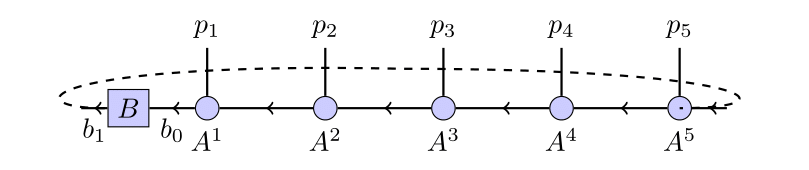
\includegraphics[width=\columnwidth]{mpsbc.png}
%    \caption{Matrix Product State with arbitrary boundary conditions}
%    \label{fig:mps_boundary}
%\end{figure}

An extension of this to treat inversion symmetry is explained in 
\onlinecite{pollmann2010}. It works identically, but instead each matrix 
product state is transposed in the basis \brayden{Add pictures for inversion 
symmetry in MPS}.



\begin{tabular*}{\columnwidth}{@{\extracolsep{\stretch{1}}}*{5}{r}@{}}
\toprule
$\mathbf{G}$ & $\mathbf{U_g}$ & $\mathbf{\theta_g}$ & $\mathbf{V_g}$ &$\mathbf{V_g V^*_g}$ \\
\midrule
 $U(1) $ & & & & \\
 $\mathcal{\pi} \mathcal{I}_x$ & & & & \\
 $\mathcal{I}_x \mathcal{I}_y$ & & & & \\
 $\mathcal{\pi} \mathcal{I}_x \mathcal{I}_y$ & & & & \\
\bottomrule
\end{tabular*}

Since 
$$  
V_{\mathcal{\pi} \mathcal{I}_y} V_{\mathcal{\pi} \mathcal{I}_y}^* = -I \text{\quad or \quad } V_{\mathcal{\pi}} V_{\mathcal{I}_y} = - V_{\mathcal{I}_y} V_{\mathcal{\pi}},
$$ 

the representation is in the nontrivial class of 

$$
H^2(\mathbb{Z}_2 \times \mathbb{Z}_2^{\mathcal{I}}; U(1)) = \mathbb{Z}_2.
$$


\newcommand{\uL}{\mathbf{L_0}}
\newcommand{\bL}{\mathbf{\bar{L}_0}}

\subsection{Identification of edge CFT}
\label{sec:CFT}

Given the $U(1)$ symmetry of the state, the simplest possible 
conformal field theory we might expect to appear at the edge is that 
of a single free bosonic field. 

The free-boson CFT is created from the Lagrangian 
$$ \mathfrak{L} = \frac{g}{2}\int dt \int\limits_0^L dx ( \frac{1}{v^2}(\partial_t \phi)^2 - (\partial_x \phi)^2)$$
and with the compatified field identification
$$ \phi \equiv \phi + 2\pi R$$
and placed on the circle of circumference $L$ with periodic boundary conditions
$$ \phi(x) \equiv \phi(x+L).$$

After canonical quantization, it is found that the set of energy 
eigenstates consists of $U(1)$ Kac-Moody primaries $\ket{e, m}$, with 
integers $e, m$ labeling the $U(1)$ charge and the winding number of 
the bosonic field respectively, and level $n, \bar{n}$ descendant 
fields for each primary - such as  $\mathbf{\bar{j}}_{-\bar{n}} 
\mathbf{j}_{-n} \ket{e, m}$ - for any nonnegative integers $n, 
\bar{n}$. The number of level $n, \bar{n}$ descendants of a given 
primary, all of which are degenerate, is $Z(n) Z(\bar{n})$, where 
$Z(n)$ is the number of partitions of the integer $n$.

The properties of the $U(1)$ Kac-Moody algebras constrain the form of 
energy and momentum eigenvalues - for the state 
$\mathbf{\bar{j}}_{-\bar{n}} \mathbf{j}_{-n} \ket{e, m}$, 

\begin{align*}
	\mathbf{P} =\frac{2\pi}{L}&(\uL-\bL) 
	&=& \frac{2\pi}{L}(em + n - \bar{n}) \\
	\mathbf{H} = \frac{2\pi}{L}&(\uL+\bL) 
	&=& \frac{2\pi}{L}(\frac{\kappa e^2}{2} + \frac{m^2}{2 \kappa} + \frac{n + \bar{n}}{2}) %\\
\end{align*}

By rescaling the energy and momentum, we find a system size 
independent pattern that can be matched to the low-energy, linearly 
dispersing part of the entanglement spectrum from Figures 
\ref{fig:ESL10} and \ref{fig:ESL9}. 

\begin{align*}
\mathbf{P} &\propto (em + n - \bar{n}) \\
\mathbf{H} &\propto e^2 + \frac{m^2}{\kappa^2} + \frac{1}{\kappa}(n + \bar{n})
\end{align*}

The label $m$ is 0 for all states in the linearly dispersing cone 
around $K=0$ - however, the primary states $\ket{e, m=\pm 1}$ can be 
found centered around momentum $K=\pi$, as seen in critical spin 
chains [reference]. The states with nonzero $e$ and zero $m$ are 
degenerate in energy and momentum with the same state with charge 
$-e$, but the $Z(n)Z(\bar{n})$ degeneracies predicted for descendant 
states are split by finite size effects.

The parameter $\kappa$ that appears - related to the coupling constant 
$g$ in the effective Lagrangian - is free. Quantum models that exhibit 
critical points that show the behavior of the free-boson CFT in fact 
have a whole line of critical points with varying values of $\kappa$, 
which can be tuned using a marginal operator in the theory.

\begin{figure}[htbc]
	\centering
	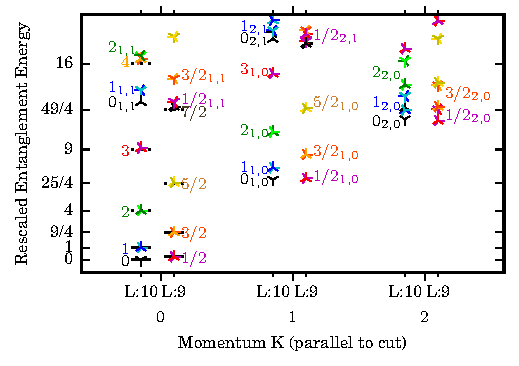
\includegraphics[width=\columnwidth]{EEIdentify.pdf}
	\caption{The identification of the primary states $\ket{\pm e, m=0}$ and the level $n, \bar{n}$ 
	descendants in the spectrum of the soft-core boson entanglement Hamiltonian. The states are labeled 
	$e_{n, \bar{n}}$. The zero and scale of the numerical spectrum are set by matching the lowest two 
	states. The energies and charges of the primaries with charges $2, 5/2, ... 4$ appear at the predicted 
	spots.  The best estimate for the Luttinger parameter from this spectrum is $\kappa \approx 1/6.4$, 
	taken from the energy of the $0_{1, 0}$ state. }
	\label{fig:EEIdentify}
\end{figure}

We can also take the lowest-lying Schmidt state, interpret it as the 
ground state of a 1d Hamiltonian, and consider its entanglement.

\begin{figure}[htbc]
	\centering
	\includegraphics[width=\columnwidth]{{EdgeGS_EntanglementEntropy.pdf}}
	\caption{Entanglement entropy within the entanglement ground state 
of the soft-core boson state on $10$ sites. For comparison, the 
Cardy-Calabrese formula $S(x) = c/3 \log \sin( \pi x/L) + const.$ is 
shown with $c=\frac{1}{2}, 1,$ and $2$, with the $const.$ fixed by 
matching the maximum of the entanglement entropy data. $c=1$ is a good 
fit.}
	\label{fig:EdgeGS_EE}
\end{figure}